
\documentclass[11pt, dvipsnames, handout]{beamer}
\newtoggle{full}
\settoggle{full}{true}

\newtoggle{covered}
\settoggle{covered}{false}

\newtoggle{presentable}
\settoggle{presentable}{false}

\newtoggle{dualscreen}
\settoggle{dualscreen}{false}

\usepackage{pgfplots}
%\pgfplotsset{compat = newest}

\usepackage{pgfpages}

\setbeamertemplate{note page}{\pagecolor{yellow!5}\vfill \insertnote \vfill}
\usepackage{collect}
\definecollection{notes}
\newcounter{notestaken}

\usepackage{xpatch}

\usepackage{ulem}

\usepackage[framemethod=tikz]{mdframed}

\usepackage{scalerel}
\usepackage{calc}

%\usepackage{enumitem}
\setlength\fboxsep{.2em}

\usepackage{graphicx} % Allows including images
\usepackage{booktabs} % Allows the use of \toprule, \midrule and \bottomrule in tables

\xpatchcmd{\itemize}
  {\def\makelabel}
  {\setlength{\itemsep}{0.65 em}\def\makelabel}
  {}
  {}


\xpatchcmd{\beamer@enum@}
  {\def\makelabel}
  {\setlength{\itemsep}{0.65 em}\def\makelabel}
  {}
  {}


%\makeatletter
%\renewcommand{\itemize}[1][]{%
%  \beamer@ifempty{#1}{}{\def\beamer@defaultospec{#1}}%
%  \ifnum \@itemdepth >2\relax\@toodeep\else
%    \advance\@itemdepth\@ne
%    \beamer@computepref\@itemdepth% sets \beameritemnestingprefix
%    \usebeamerfont{itemize/enumerate \beameritemnestingprefix body}%
%    \usebeamercolor[fg]{itemize/enumerate \beameritemnestingprefix body}%
%    \usebeamertemplate{itemize/enumerate \beameritemnestingprefix body begin}%
%    \list
%      {\usebeamertemplate{itemize \beameritemnestingprefix item}}
%      {%
%        \setlength\topsep{1em}%NEW
%        \setlength\partopsep{1em}%NEW
%        \setlength\itemsep{1em}%NEW
%        \def\makelabel##1{%
%          {%
%            \hss\llap{{%
%                \usebeamerfont*{itemize \beameritemnestingprefix item}%
%                \usebeamercolor[fg]{itemize \beameritemnestingprefix item}##1}}%
%          }%
%        }%
%      }
%  \fi%
%  \beamer@cramped%
%  \raggedright%
%  \beamer@firstlineitemizeunskip%
%}
%
%
%
%
%
%\makeatother

%\setlist[beamer@enum@]{topsep=1 em}
%\let\origcheckmark\checkmark %screw you dingbat
%\let\checkmark\undefined %screw you dingbat
%\usepackage{dingbat} 
%\let\checkmark\origcheckmark %screw you dingbat






%\usepackage{fontawesome}

\usepackage{mathtools}
\usepackage{etoolbox, calculator}

\usepackage{xcolor}
\usepackage{tikz}
\usetikzlibrary{arrows.meta}
\usetikzlibrary{calc}
\usepackage[nomessages]{fp}
\usepackage{transparent}
\usepackage{accsupp}
%\usepackage{color, xcolor}

%colorblind-friendly palette
%\definecolor{dblue}{RGB}{51,34,136}
\definecolor{lblue}{RGB}{136,204,238}
%\definecolor{green}{RGB}{17,119,51}
\definecolor{tan}{RGB}{221,204,119}
%\definecolor{mauve}{RGB}{204,102,119}

\usepackage{tcolorbox}



\usepackage{xifthen}
\usepackage{nicefrac}
\usepackage{amsmath}
\usepackage{amsthm}
\usepackage{amssymb}
\theoremstyle{definition}
\newtheorem*{define}{Definition}
\newtheorem*{recall}{Recall}


\DeclareMathOperator{\tr}{tr}

\usepackage{multicol}
%\setlength{\columnsep}{1cm}

\usepackage{tablists, amsmath,vwcol, cancel, polynom}
\usetikzlibrary{shapes, patterns, decorations.shapes}
%\usepackage{tikzpeople}
\tikzstyle{vertex}=[shape=circle, minimum size=2mm, inner sep=0, fill]
\tikzstyle{opendot}=[shape=circle, minimum size=2mm, inner sep=0, fill=white, draw]

% common math quick commands
\newcommand{\nicedd}[2]{\nicefrac{\text{d}#1}{\text{d}#2}}
\newcommand{\dd}[2]{\dfrac{\text{d}#1}{\text{d}#2}}
\newcommand{\pd}[2]{\dfrac{\partial #1}{\partial#2}}
\renewcommand{\d}[1]{\text{d}#1}
\newcommand{\ddn}[3]{\dfrac{\text{d}^{#3}#1}{\text{d}#2^{#3}}}
\newcommand{\pdn}[3]{\dfrac{\partial^{#3}#1}{\partial#2^{#3}}}
\newcommand{\p}[0]{^{\prime}}
\newcommand{\pp}[0]{^{\prime\prime}}
\newcommand{\op}[2][\text{L}]{#1 \left[ #2 \right]}

\newcommand{\lap}[1]{\mathcal{L}\left\{#1\right\}}
\newcommand{\lapinv}[1]{\mathcal{L}^{-1}\left\{#1\right\}}
\newcommand{\lapint}[1]{\int_0^\infty e^{-st}#1dt}
\newcommand{\evalat}[2]{\Big|_{#1}^{#2}}

\newcommand{\paren}[1]{ \left( #1 \right)}

\newcommand{\haxis}[4][\normcolor]{\draw[#1, <->] (-#2,0)--(#3,0) node[right]{$#4$}; }


\newcommand{\axis}[4]{\draw[\normcolor, <->] (-#1,0)--(#2,0) 
node[right]{$x$};
\draw[help lines, <->] (0,-#3)--(0,#4) node[above]{$y$};}

\newcommand{\laxis}[6]{\draw[<->] (-#1,0)--(#2,0) 
node[right]{$#5$};
\draw[ <->] (0,-#3)--(0,#4) node[above]{$#6$};}
\newcommand{\xcoord}[2]{
	\draw (#1,.2)--(#1,-.2) node[below]{$#2$};}
\newcommand{\textnode}[3]{
	\draw (#1,#2) node[below]{$#3$};}
	
\newcommand{\nxcoord}[2]{
	\draw (#1,-.2)--(#1,.2) node[above]{$#2$};}
\newcommand{\ycoord}[2]{
	\draw (.2,#1)--(-.2,#1) node[left]{$#2$};}
\newcommand{\nycoord}[2]{
	\draw (-.2,#1)--(.2,#1) node[right]{$#2$};}
\newcommand{\dlim}{\displaystyle\lim}
\newcommand{\dlimx}[1]{\displaystyle\lim_{x \rightarrow #1}}
\newcommand{\stickfig}[2]{
	\draw (#1,#2) arc(-90:270:2mm);
	\draw (#1,#2)--(#1,#2-.5) (#1-.25,#2-.75)--(#1,#2-.5)--(#1+.25,#2-.75) (#1-.2,#2-.2)--(#1+.2,#2-.2);}	

%\newcounter{example}
%\setcounter{example}{1}
%\newcounter{preFrameExample}
%\AtBeginEnvironment{frame}{\setcounter{preFrameExample}{\value{example}}}
%\newcommand{\ex}[1]{
%	 \setcounter{example}{\value{preFrameExample}}
%	 \textcolor{green}{\small\fbox{Example \arabic{example}: #1}}\\[8pt]
%	\stepcounter{example}}
%\newcommand{\exans}[1]{
%	\SUBTRACT{\value{preFrameExample}}{1}{\n}
%	 \textcolor{green}{\small\fbox{Solution \n: #1}}\\[8pt]}
\mode<presentation> {

% The Beamer class comes with a number of default slide themes
% which change the colors and layouts of slides. Below this is a list
% of all the themes, uncomment each in turn to see what they look like.


\usetheme{CambridgeUS}
\usecolortheme[named=black]{structure}


\newcommand{\studentcolor}[0]{ForestGreen}
\newcommand{\normcolor}[0]{NavyBlue}
\newcommand{\alertcolor}{Red}

\setbeamercolor{normal text}{fg=\normcolor}
\setbeamercolor{frametitle}{fg=\normcolor}
\setbeamercolor{section in head/foot}{fg=Black, bg=Gray!20}
\setbeamercolor{subsection in head/foot}{fg=Green!70!Black, bg=Gray!10}
\setbeamercolor{alerted text}{fg=\alertcolor}
\setbeamerfont{alerted text}{series=\bf}
\setbeamertemplate{enumerate items}[default]
\setbeamercolor{enumerate item}{fg=\normcolor}

\setbeamertemplate{footline} % To remove the footer line in all slides uncomment this line
%\setbeamertemplate{footline}[page number] % To replace the footer line in all slides with a simple slide count uncomment this line

\setbeamertemplate{navigation symbols}{} % To remove the navigation symbols from the bottom of all slides uncomment this line
}

\newcommand{\alertbox}[1]{\tcbox[on line, colframe=\alertcolor, colback=White, left=2pt,right=2pt,top=2pt,bottom=2pt]{\usebeamercolor*{normal text}#1}}


\newcommand{\startstu}{\setbeamercolor{normal text}{fg=\studentcolor}\usebeamercolor*{normal text}\setbeamercolor{enumerate item}{fg=\studentcolor}\usebeamercolor*{enumerate item}}
\newcommand{\stopstu}{\setbeamercolor{normal text}{fg=\normcolor}\usebeamercolor*{normal text}\setbeamercolor{enumerate item}{fg=\normcolor}\usebeamercolor*{enumerate item}}

\newcommand{\takenote}[1]{ \begin{collect}{notes}{}{}{}{}  #1  \end{collect}  \addtocounter{notestaken}{1}} %\ifthenelse{\value{notestaken}>0}{\hrulefill\\}{}

\makeatletter
\newcommand{\cover}{\alt{\beamer@makecovered}{\beamer@fakeinvisible}}
\newcommand{\ucover}[1]{\iftoggle{full}{}{\beamer@endcovered}\stopstu#1\startstu\iftoggle{full}{}{\beamer@startcovered}}
\makeatother

\newcommand{\skippause}{ \addtocounter{beamerpauses}{-1}}
\newcommand{\blockpres}{ \skippause \pause }

\newcommand{\studentify}[1]{\startstu #1  \stopstu }
\newcommand{\student}[1]{\iftoggle{full}{ \pause  \studentify{#1} }{\iftoggle{covered}{\studentify{#1}}{\cover{  #1 }}}}
\newcommand{\cstudent}[1]{\student{\begin{center} #1 \end{center}}}
\newcommand{\fullonly}[1]{\iftoggle{full}{ #1}{}}
\newcommand{\presentonly}[1]{\iftoggle{presentable}{ #1}{}}

\usepackage{xparse}
\usepackage{xifthen}

% shortcuts for commonly-used presentation elements
%\NewDocumentCommand{\slide}{o m}
% {\IfValueTF{#1}{\begin{frame}[t]{#1}}{\begin{frame}[t]} #2 \end{frame}}

\newtoggle{iscovered}

\newcommand{\slide}[2][]{%
%\setcounter{notestaken}{0}
\takenote{#2} 
%\ifthenelse{\equal{#1}{}}{\begin{frame}[t]}{\begin{frame}[t]{#1}} #2 \ifthenelse{\value{notestaken}>0}{ \note{\includecollection{notes}}}{} \end{frame}%
\ifthenelse{\equal{#1}{}}{\begin{frame}[t]}{\begin{frame}[t]{#1}} #2 \iftoggle{covered}{\settoggle{iscovered}{true}}{\settoggle{iscovered}{false}}  \note{ \iftoggle{iscovered}{}{\settoggle{covered}{true}} #2 \iftoggle{iscovered}{}{\settoggle{covered}{false}} } \end{frame}%
%\setcounter{notestaken}{0}
}
\newcommand{\defn}[2][]{%
 \setcounter{listcounter}{0}%
\ifthenelse{\equal{#1}{}}{\begin{block}{Definition}}{\begin{block}{#1 :}}%
 #2 \vspace{0.25em} \ifthenelse{\value{listcounter}>0}{\skippause}{} \pause \end{block}%
}



\newcommand{\arr}[2]{\begin{array}{#1}#2\end{array}}
\newcommand{\mat}[2]{\left[\arr{#1}{#2}\right]}
\newcommand{\carray}[1]{\arr{c}{#1}}
\newcommand{\larray}[1]{\arr{l}{#1}}
\newcommand{\rarray}[1]{\arr{r}{#1}}
\newcommand{\colvec}[1]{\mat{c}{#1}}

\newcommand{\itmz}[1]{\addtocounter{listcounter}{1} \begin{itemize}#1 \end{itemize} }
\newcommand{\subitem}[1]{\addtocounter{listcounter}{1} \begin{itemize} \item #1 \end{itemize}}
%
\newcommand{\enum}[1]{\addtocounter{listcounter}{1} \begin{enumerate} #1  \end{enumerate}  }


\newcommand{\algnlbl}[1]{\begin{align}#1  \end{align}} 
\newcommand{\algn}[1]{\begin{align*}#1  \end{align*}} 
\newcommand{\lgn}[1]{ \action<+->{#1} }
\newcommand{\slgn}[1]{\iftoggle{full}{\action<+->{ \startstu #1 \stopstu}}{ \cover{ #1 } } \takenote{$#1$}}

\newcommand{\chckmrk}{\alert{\checkmark}}

\usepackage{pifont}
\newcommand{\xmark}{\alert{\text{\large \ding{55}}}}

\newcommand{\return}[0]{\raisebox{.5ex}{\rotatebox[origin=c]{180}{$\Lsh$}}}
\usepackage{pbox}
%\newcommand{\ex}[1]{\rotatebox[origin=c]{10}{\uline{ex}}:$\;$\pbox[t][][b]{0.9\linewidth}{#1}}
\newcommand{\ex}[1]{\uline{ex}:$\;$\pbox[t][][t]{0.9\linewidth}{#1}}
\newcommand{\eg}[1]{e.g.,$\;$\pbox[t][][t]{0.9\linewidth}{#1}}
\newcommand{\tikzplot}[8][]{%
\begin{tikzpicture}

\begin{scope}[]%
\clip(-#2,-#4) rectangle (#3,#5);%
#8%
\end{scope}%
\laxis{#2}{#3}{#4}{#5}{#6}{#7}%
#1
\end{tikzpicture}%
}


\newcommand{\cancelslide}[1]{%
\begingroup%
\setbeamertemplate{background canvas}{%
\begin{tikzpicture}[remember picture,overlay]%
\draw[line width=2pt,red!60!black] %
  (current page.north west) -- (current page.south east);%
\draw[line width=2pt,red!60!black] %
  (current page.south west) -- (current page.north east);%
\end{tikzpicture}}%
#1%
\endgroup%
}
\renewcommand{\CancelColor}{\color{red}}
\newcommand{\twocols}[3][0.5]{\begin{columns}\begin{column}{#1\textwidth}#2\end{column}\hspace{1em}\vrule{}\hspace{1em}\begin{column}{#1\textwidth}#3\end{column}\end{columns}}

\newcommand{\twomini}[5][1]{\calculatespace \begin{minipage}[t]{\columnwidth}\begin{minipage}[][#1\contentheight][t]{#2\columnwidth}#4\end{minipage}\hfill\begin{minipage}[][#1\contentheight][t]{#3\columnwidth}#5\end{minipage}\end{minipage}}

\newcommand{\threemini}[7][1]{\calculatespace \begin{minipage}[t]{\columnwidth}\begin{minipage}[][#1\contentheight][t]{#2\columnwidth}#5\end{minipage}\hfill\begin{minipage}[][#1\contentheight][t]{#4\columnwidth}#6\end{minipage}\hfill\begin{minipage}[][#1\contentheight][t]{#3\columnwidth}#7\end{minipage}\end{minipage}}


\newcounter{listcounter}
\setcounter{listcounter}{0}



\newif\ifsidebartheme
\sidebarthemetrue

\newdimen\contentheight
\newdimen\contentwidth
\newdimen\contentleft
\newdimen\contentbottom
\makeatletter
\newcommand*{\calculatespace}{%
\contentheight=\paperheight%
\ifx\beamer@frametitle\@empty%
    \setbox\@tempboxa=\box\voidb@x%
  \else%
    \setbox\@tempboxa=\vbox{%
      \vbox{}%
      {\parskip0pt\usebeamertemplate***{frametitle}}%
    }%
    \ifsidebartheme%
      \advance\contentheight by-1em%
    \fi%
  \fi%
\advance\contentheight by-\ht\@tempboxa%
\advance\contentheight by-\dp\@tempboxa%
\advance\contentheight by-\beamer@frametopskip%
\ifbeamer@plainframe%
\contentbottom=0pt%
\else%
\advance\contentheight by-\headheight%
\advance\contentheight by\headdp%
\advance\contentheight by-\footheight%
\advance\contentheight by4pt%
\contentbottom=\footheight%
\advance\contentbottom by-4pt%
\fi%
\contentwidth=\paperwidth%
\ifbeamer@plainframe%
\contentleft=0pt%
\else%
\advance\contentwidth by-\beamer@rightsidebar%
\advance\contentwidth by-\beamer@leftsidebar\relax%
\contentleft=\beamer@leftsidebar%
\fi%
}
\makeatother


\iftoggle{dualscreen}{\setbeameroption{show notes on second screen=right}}{}


\begin{document}
\section{Lecture 24}
\subsection{Introduction}

\slide[ Homogeneous Heat Equation]{\vspace{-2.5em}
\algn{\larray{u_t= \alpha u_{xx}\\\text{for } x\in[0,L]} \; \text{with }& \larray{u(0,t)=u(L,t)=0 \\ \qquad \qquad \qquad  \text{\uline{or}} \\ u_x(0,t)=u_x(L,t)=0} &\text{and}\quad  &u(x,0)=u_0(x)}
\vfill
\[\boxed{u(x,t)=\frac{a_0}{2} + \sum_{n=1}^\infty e^{-\alpha \frac{n^2\pi^2}{L^2} t} \left( a_n \cos\left(\frac{n\pi}{L} x\right) +  b_n \sin\left(\frac{n\pi}{L} x\right) \right)  }\]\vfill
\twomini[.45]{.5}{.5}{
 \uline{$u(0,t)=u(L,t)=0$}: $\quad$\vfill
Fourier sine series
\small 
\algn{a_n &= 0\\b_n&=\frac{2}{L}\int_0^L u_0(x) \sin\paren{\frac{n\pi}{L}x} dx }
}{
\uline{$u_x(0,t)=u_x(L,t)=0$}: \vfill 
Fourier cosine series
\small
\algn{a_n &= \frac{2}{L}\int_0^L u_0(x) \cos\paren{\frac{n\pi}{L}x} dx\\b_n&=0 }
}
}
\subsection{Behaviour of Solutions}
\slide[]{
The heat equation smooths out initial conditions.
\vfill
\ex{$u_0(x)=u_{\frac{L}{4}}(x)-u_{\frac{3L}{4}}(x) = H\paren{x-\frac{L}{4}} - H\paren{x-\frac{3L}{4}}$}\vfill
\twomini[.7]{.5}{.5}{
 \uline{$u(0,t)=u(L,t)=0$}: \vfill
\centerline{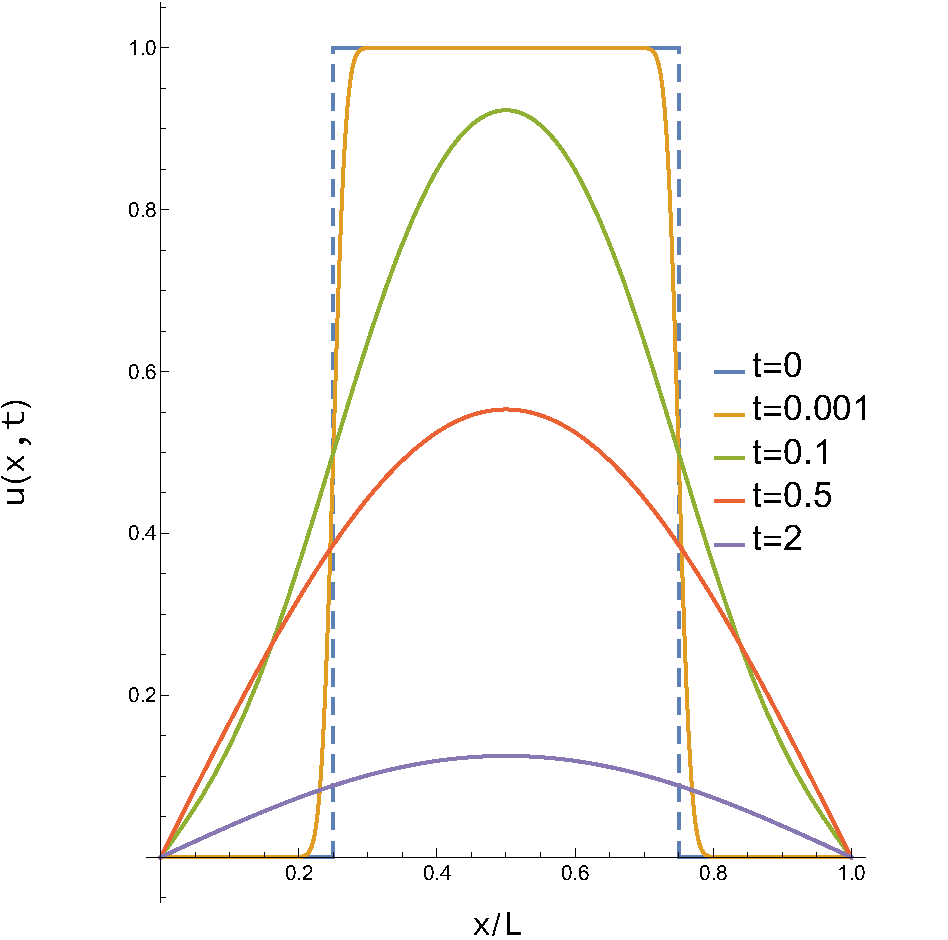
\includegraphics[width=0.9\columnwidth]{images/clamped_BCs_heaviside.pdf}}
}{
 \uline{$u_x(0,t)=u_x(L,t)=0$}: \vfill
\centerline{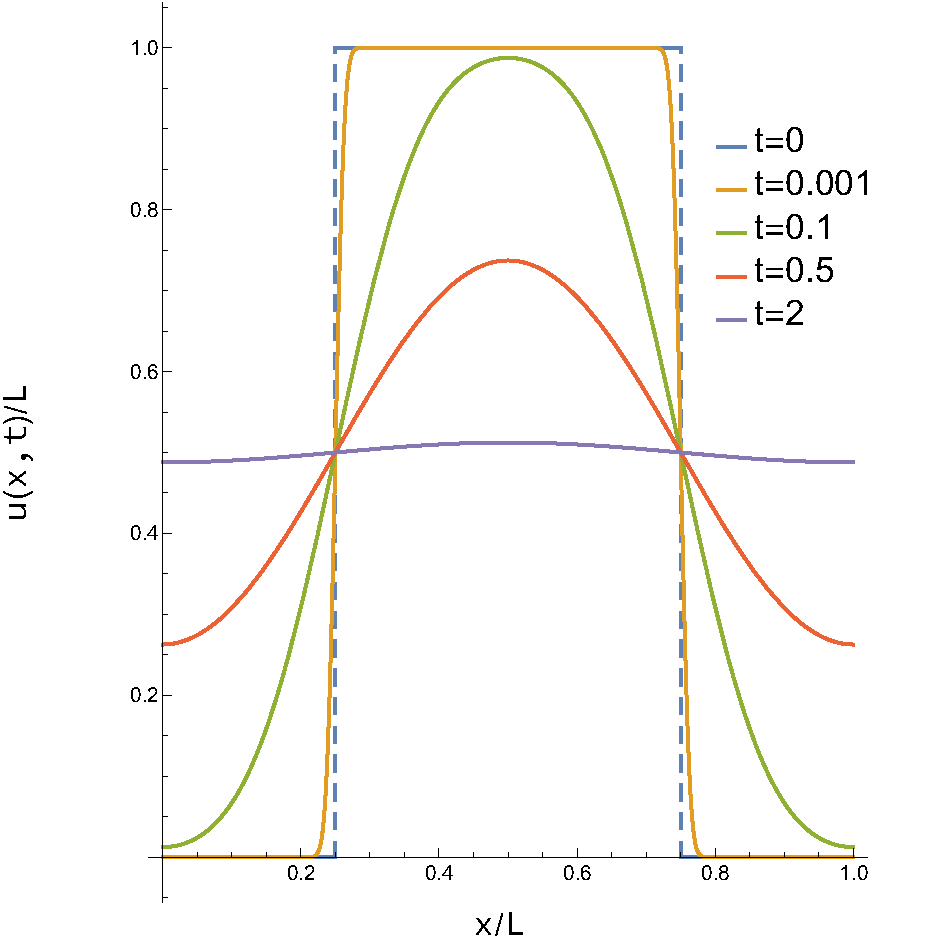
\includegraphics[width=0.9\columnwidth]{images/zero_flux_BCs_heaviside.pdf}}}
}

\slide[Short-term Behaviour]{\vspace{-2em}
\[ u(x,t) =\frac{a_0}{2} + \sum_{n=1}^\infty\underbrace{ e^{-\alpha \frac{n^2\pi^2}{L^2} t}}_{\larray{\\\text{Exp. Decay}}} \cdot \; \underbrace{ \left( a_n \cos\left(\frac{n\pi}{L} x\right) +  b_n \sin\left(\frac{n\pi}{L} x\right) \right)}_{\text{$n^{th}$ Fourier Mode}}  \]
\vfill
\twomini[.7]{.45}{.55}{
\centerline{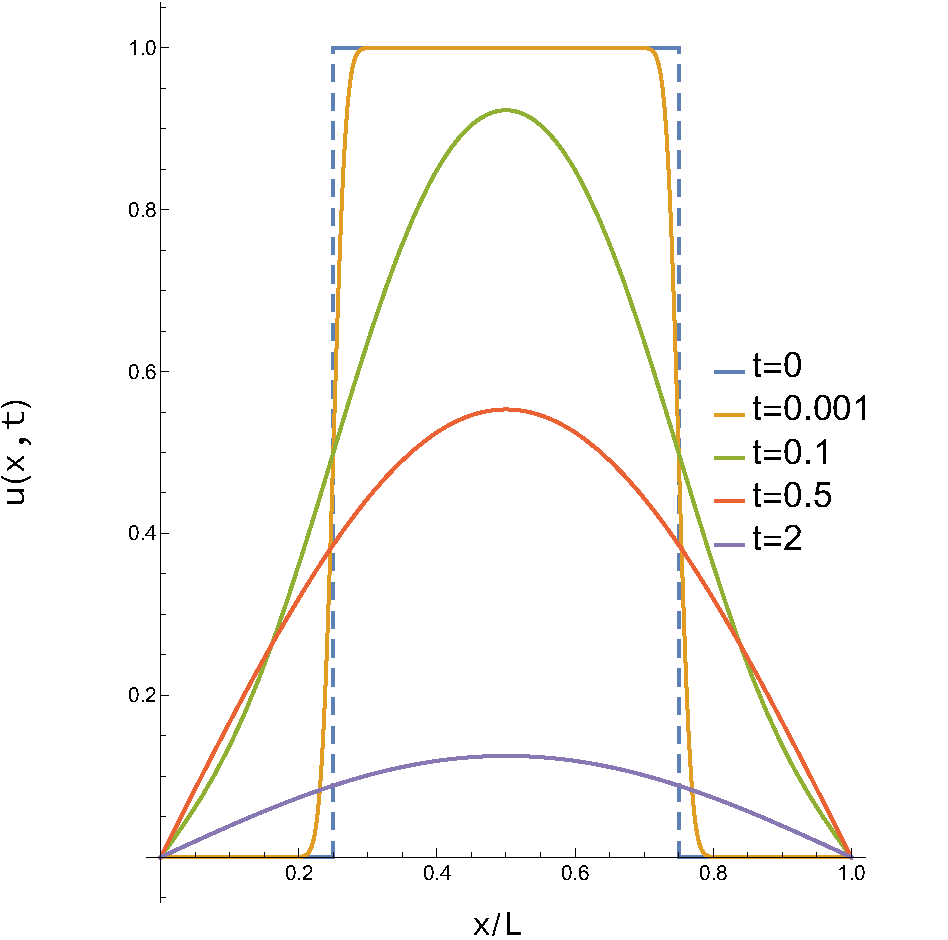
\includegraphics[width=\columnwidth]{images/clamped_BCs_heaviside.pdf}}
}{
\student{
\itmz{\item Sharp edges in the initial condition require high frequncy modes ($n\gg1$).
\item The exp. decay rate grows with $n^2$.
\item High frequency modes decay the fastest. 
\item Sharp features get smoothed out very quickly.

}
}
}
}

\subsection{Asymptotic Approximation}
\slide[Long-term Behaviour]{
As $t\to\infty$,
\algn{
\lim_{t\to\infty} u(x,t) &=\frac{a_0}{2} + \sum_{n=1}^\infty e^{-\alpha \frac{n^2\pi^2}{L^2} t} \left( a_n \cos\left(\frac{n\pi}{L} x\right) +  b_n \sin\left(\frac{n\pi}{L} x\right) \right) \\
&=\frac{a_0}{2}} 

For finite $t\gg0$, we can just keep the first non-zero term in the infinite sum. All other terms decay much much faster.
\vfill
\twomini[.25]{.5}{.5}{
 \uline{$u(0,t)=u(L,t)=0$}: $\quad$\vfill

\small 
\[u(x,t) \approx e^{-\alpha \frac{\pi^2}{L^2}t}b_1\sin\paren{\frac{\pi}{L}x} \]
}{
\uline{$u_x(0,t)=u_x(L,t)=0$}: \vfill 
\small
\[u(x,t) \approx \frac{a_0}{2} + e^{-\alpha \frac{\pi^2}{L^2}t}a_1\cos\paren{\frac{\pi}{L}x} \]
}
}


\slide{
\uline{$u(0,t)=u(L,t)=0$}: $u(x,t) \approx e^{-\alpha\frac{\pi^2}{L^2}t}b_1\sin\paren{\frac{\pi}{L}x}$\vfill 
\centerline{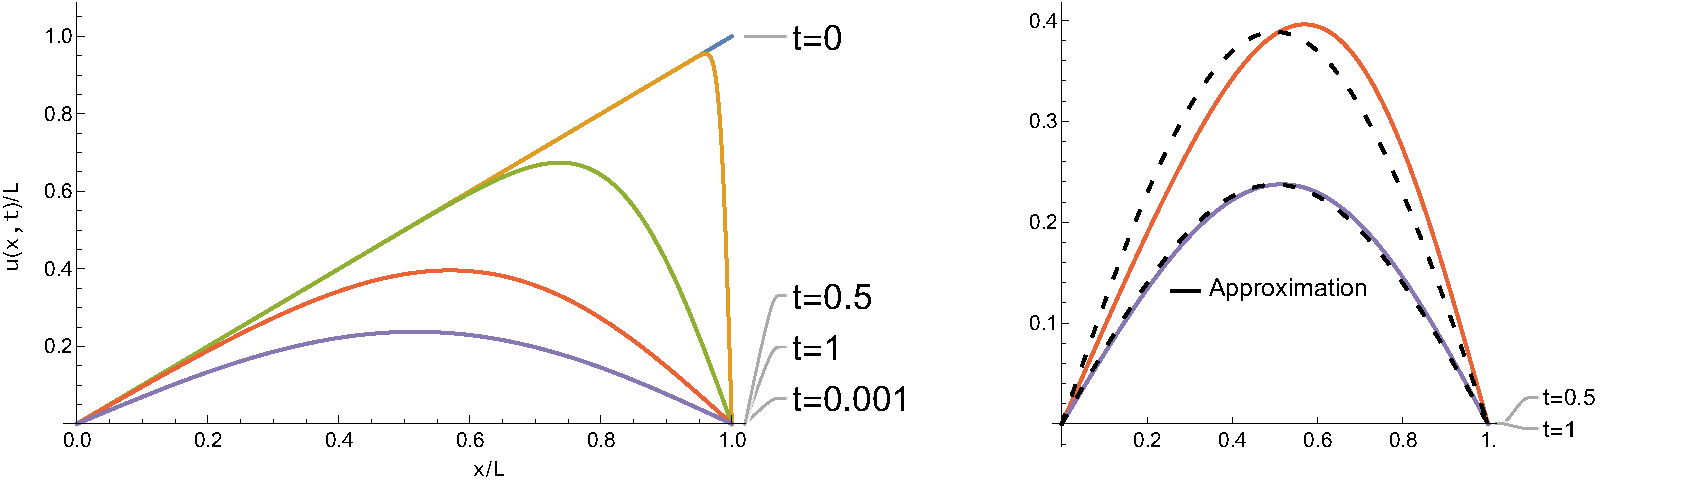
\includegraphics[width=12cm]{images/clamped_BCs_long_term.pdf}}\vfill
\uline{$u_x(0,t)=u_x(L,t)=0$}: $u(x,t) \approx \frac{a_0}{2} + e^{-\alpha\frac{\pi^2}{L^2}t}a_1\cos\paren{\frac{\pi}{L}x} $ \vfill 
\centerline{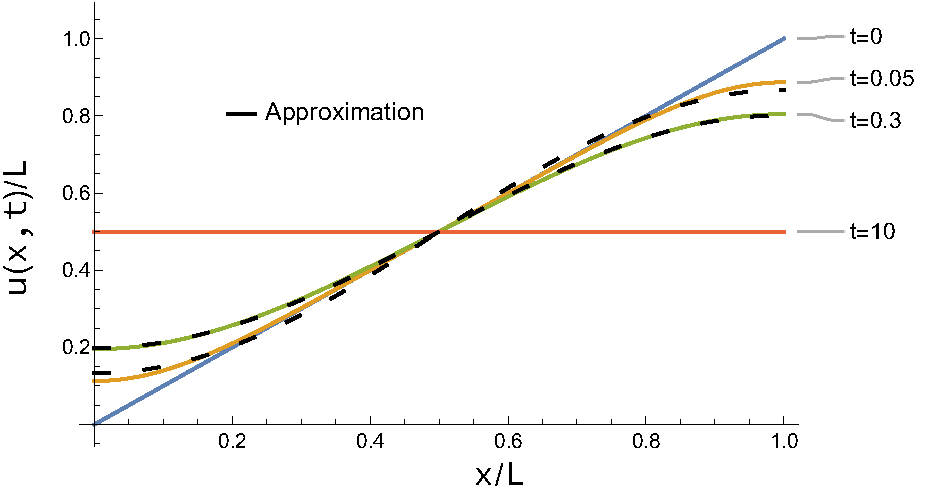
\includegraphics[width=7cm]{images/zero_flux_BCs_long_term.pdf}}

}


\slide{
\ex{\twomini[.1]{.7}{.295}{$u_t=\alpha u_{xx}$, \hspace{2em} $\arr{l}{u(0,t)=u(1,t)=0 \hspace{1em}\\u(x,0)=x(1-x) \text{ on } [0,1]}$}{\tikzplot[\xcoord{2}{\scriptscriptstyle 1}]{.1}{2.1}{.1}{1}{x\phantom{t}}{\scriptscriptstyle u(x,0)}{\draw[domain=0:1] plot (2*\x,{3*\x*(1-(\x))});}}\hfill}
\vfill
\student{
BCs $\Rightarrow$ only $\sin$ terms survive.\vspace{-.75em}
\algn{u(x,t)&=\sum_{n=1}^\infty b_n \sin(n \pi x)e^{-\alpha n^2\pi^2 t}\\
u(x,0) &=\sum_{n=1}^\infty b_n \sin(n \pi x) =x(1-x)\\
b_n&=\frac{2}{1} \int_0^1 u(x,0)\sin(n\pi x)dx=2 \int_0^1 x(1-x)\sin(n\pi x)dx\\
&\overset{\text{wolfram}}{=} 2\paren{\frac{-2((-1)^n-1)}{n^3\pi^3}}\qquad  \Rightarrow \qquad \boxed{ b_n =-\frac{4}{\pi^3}\frac{(-1)^{n}-1}{n^3}}}
}\vfill
\tiny
\url{https://www.wolframalpha.com/input?i=integral+of+x\%281-x\%29sin\%28n*pi*x\%29+from+0+to+1+assuming+n+is+an+integer}
}%end slide

\slide{Given \[u(x,t)=-\sum_{n=1}^\infty \frac{4}{\pi^3}\frac{(-1)^{n}-1}{n^3}  \sin(n \pi x)e^{-\alpha n^2\pi^2 t}\]  suppose that after 100 time units the hottest point in the domain is at half of its initial temperature, find an approximation for $\alpha$.
\student{
\algn{\text{Initial Condition: }u_0(x)&=x(1-x) \\\Rightarrow x_{\rm max} &= \frac12 &u_0(x_{\rm max})&=\frac14\\
\text{Long-term: } u(x,t) &\approx  \frac{8}{\pi^3}  \sin( \pi x) e^{-\alpha \pi^2 t} \intertext{approximation also has its max at $x=1/2$}
 \frac{8}{\pi^3}  e^{-\alpha \pi^2 100 }& \approx \frac18 & \alpha &\approx -\frac{1}{100 \pi^2} \log\left(   \frac{\pi^3}{64}\right)\\
&&\alpha&\approx 7.34\times10^{-4}
}
}
}

\slide{
\ex{\twomini[.1]{.7}{.295}{$u_t=0.1 u_{xx}$, \hspace{2em} $\arr{l}{u_x(0,t)=u_x(1,t)=0 \hspace{1em}\\u(x,0)=x(1-x) \text{ on } [0,1]}$}{\tikzplot[\xcoord{2}{\scriptscriptstyle 1}]{.1}{2.1}{.1}{1}{x\phantom{t}}{\scriptscriptstyle u(x,0)}{\draw[domain=0:1] plot (2*\x,{3*\x*(1-(\x))});}}\hfill}
\vfill
\student{
BCs $\Rightarrow$ only $\cos$ terms survive.\vspace{-.75em}
\algn{u(x,t)&=\sum_{n=1}^\infty a_n \sin(n \pi x)e^{-0.1 n^2\pi^2 t}\\
u(x,0) &=\sum_{n=1}^\infty a_n \sin(n \pi x) =x(1-x)\\
a_n&=\frac{2}{1} \int_0^1 u(x,0)\cos(n\pi x)dx=2 \int_0^1 x(1-x)\sin(n\pi x)dx\\
&\overset{\text{wolfram}}{=} -2\frac{(-1)^n+1}{\pi^2 n^2}\\
a_0&=\frac{2}{1}\int_0^1 x(1-x)dx = \frac{2}{6}}
}\vfill
\tiny
\url{https://www.wolframalpha.com/input?i=integral+of+x\%281-x\%29cos\%28n*pi*x\%29+from+0+to+1+assuming+n+is+an+integer}\vfill
\url{https://www.wolframalpha.com/input?i=integral+of+x\%281-x\%29+from+0+to+1}
}%end slide

\slide{Given \[u(x,t)= \frac16 - 2 \sum_{n=1}^\infty  \frac{(-1)^n+1}{\pi^2 n^2} \cos(n \pi x)e^{-0.1 n^2\pi^2 t}\] approximately how long does it take for the endpoints of the domain to be within 1\% of their steady state value?\\
\student{
$n=1$ has a coefficient of zero, use $n=2$ instead for approximation.
\algn{\text{Long-term: } u(x,t) &\approx  \frac16 -2\frac{2}{4\pi^2}  \ \cos( 2 \pi x) e^{-0.4 \pi^2 t}\\
 \text{Steady state: } u_{\infty}(x) &= \frac{1}{6}\\
u_\infty(x) -u(L,t) &\approx  \frac{1}{\pi^2}   \cos(2 \pi x) e^{-0.4 \pi^2 t}\\
\text{$x=0$ or $x=1$: }& \frac{1}{\pi^2}   e^{-0.4 \pi^2 t} \approx  1\%\times\frac16\\
t&\approx-\frac{1}{0.4\pi^2}\log\paren{\frac{0.01\pi^2}{6}}\\
&\approx 1.04 \text{ time units}
}
}
}


\end{document}